\chapter{Data Analysis Techniques}

\section{Fitting}\label{sec:fitting_theory}

The distributions of observables that are measured experimentally always contain, at the very least, a degree of statistical uncertainty.
In Physics, we usually model processes with smooth distributions, which can be parametrised with a set of numbers. 
\textit{Fitting} is a process of extraction of parameters from observed distributions. 
It is one of the key tasks of statistical analyses and, consequentially, particle physics measurements. 
Nearly every particle physics analysis features some kind of fitting for the result extraction. 
It is also present in particle trajectory reconstruction algorithms, calorimeter cluster shape parametrisation, and calibration procedures.
One of the most common examples is the fitting of a particle species invariant mass distribution reconstructed from its decay products.
It was, for example, used in some of the most precise of the Higgs boson mass measurements \cite{ATLAS:2018tdk,CMS:2020xrn}, in the $\H\ra\Z\Zstar\ra 4\ell$ and $\H\ra\g\g$ decay channels.

Fitting consists of two main steps: point estimation and uncertainty (confidence-interval) estimation. 
In the former, a best estimate for a set of parameters is derived, which describes a given dataset.
The latter sets the confidence interval on each parameter estimate in the set. 

The overview here presents only a brief overview of the most relevant method that was used in the work presented in this thesis. 
For a more in-depth consideration of statistical methods in data science and physics, I refer the readers to Refs. \cite{Behnke:2013pga,Blobel_Lohrmann_1998} and for rigorous proofs of the underlying statistical concepts, Refs. \cite{Bohm:2014vmk,James_2006,Barlow:1990vc}. 
The material presented here only summarises the details in these books and articles.

\subsection{Maximum-likelihood method}\label{sec:mle}

One of the most common and popular methods for parameter estimation is the maximum-likelihood method. 
It is also used here widely in this analysis, described in \Cref{ch:analysis}.

An observed dataset can be defined as $x = (x_1, x_2,...,x_N)$, with $x_i$ being the result of $N$ independent measurements following an unknown probability density $f(x)$, and $i\in[0,N]$.
The function $f(x)$ is, usually, not known and the shape is often parametrised as $f(x; a)$, where $a=(a_1,...,a_M)$ is a dimension-$M$ vector of unknown-valued parameters. 
For a fitting procedure, one has to construct an \textit{estimator}, which is a function of the observed data that can provide an estimated numerical value, $\hat{a}$, corresponding to the parameter vector $a$.
% Any estimator should satisfy four main criterion:

% \begin{itemize}
%     \item \textbf{Consistency}: as the number of measurements increases, the precision of the estimator increases, i.e.:
%      \begin{equation}
%         \lim_{N\ra\infty}\hat{a} = a,
%      \end{equation}
%     \item \textbf{Bias}: the expectation value of the estimator should be close to the true value of $a$. 
%     If the difference, $b$, is small, it is known as an unbiased estimator:
%     \begin{equation}
%         E[\hat{a}] = a + b,
%     \end{equation}
%     \item \textbf{Efficiency}: The variance of the estimator, $V[\hat{a}]$, should be small. 
%     More formally speaking it should be higher than the inverse of Fisher information, $I(a)$. This is also known as the minimum-variance bound.
%     \begin{equation}
%         V[\hat{a}] \geq \frac{1}{I(a)} \quad \mathrm{with} \quad I_{jk}(a) = -E\left[\sum^N_{i=1}\pdv{f(x_i;a)}{a_j}{a_k}\right],
%     \end{equation}
%     \item \textbf{Robustness}: against wrong inputs or incorrect assumptions.
% \end{itemize}
%Usually, it is difficult to choose an estimator that can satisfy all of these criterion simultaneously. One common estimator is the maximum-likelihood estimator.

A very common technique for an estimator is the so-called maximum-likelihood estimate, which uses the likelihood function.
The likelihood function is built from one- or multi-dimensional PDFs $f(x;a)$ of the measured values $x$:
\begin{equation}\label{eq:likelihood_equation}
    \mathcal{L}(x;a) = \prod_{i=1}^N f(x_i; a).
\end{equation}
% The PDFs used to construct the likelihood function have to be normalised, which implies that the integral of the likelihood function is independent of parameters $a$:
% \begin{equation}
%     \int f(x;a)dx = 1 \quad \ra \quad \int \mathcal{L}(x;a)dx_1dx_2...dx_N = 1.
% \end{equation}
In this case, the maximum-likelihood estimate of the parameters $a$ correspond to $\hat{a}$ for which $\mathcal{L}(x;a)$ is globally maximised.
Because the product of a large number of components can vary over many orders of magnitude, in real-life applications it is more convenient to work with sums.
Therefore, a log-likelihood function is used in practice:
\begin{equation}
    l(x;a) \equiv \ln\mathcal{L}(x;a) = \sum_{i=1}^N \ln f(x_i;a).
\end{equation}
It is worthwhile to note that a logarithm is a monotonic function, therefore the maximum of a function is the same as the maximum of its logarithm. 
The maximum of the log-likelihood function satisfies the standard requirement for an extremum point:

\begin{equation}\label{eq:likelihood_derivative}
    \pdv{l(x;a)}{a_j}=0 \quad \mathrm{for} \quad j=1,...,M.
\end{equation}
The roots of \Cref{eq:likelihood_derivative} are maximum-likelihood estimates of $\hat{a}$. Generally, it is impossible to find an extremum in a large parameter space using analytical methods.
In practice, numerical procedures and dedicated software packages for optimisation are usually used.
Many optimisers used in modern day computers tend to minimise functions, rather than maximise them, therefore a \textit{negative log-likelihood} function is often used.
Maximum-likelihood method is unbiased and consistent as the number of measurements grows, i.e. $N\ra\infty$.
However, it requires a good prior knowledge of the form of the PDF $f(x;a)$, as otherwise the result might be incorrect.

\subsection{Variance of the maximum-likelihood method}\label{sec:mle_variance}


The likelihood function generally can have any non-Gaussian shape, however it can be shown~\cite{James_2006} that in the asymptotic limit, $N\ra\infty$, 
any given $f(x;a)$ can have its likelihood function approximated with a multivariate Gaussian distribution:

\begin{equation}
    \mathcal{L} \propto \exp{-\frac{1}{2}(a-\hat{a})^T H(a-\hat{a})},
\end{equation}
where $H$ is the Hessian matrix of the log-likelihood function. Assuming a good minimum is found (\Cref{eq:likelihood_equation}), the log-likelihood function can be expanded at $a=\hat{a}$ and approximated as a parabola:
\begin{equation}
    l(x;a_1,a_2,...,a_N) = l(x;\hat{a}_1,\hat{a}_2,...,\hat{a}_N) + \frac{1}{2}\sum_{i,k} \pdv{l}{a_i}{a_k} (a_i-\hat{a}_i)(a_k-\hat{a}_k)+...
\end{equation}
In this case, the covariance matrix, $V(\hat{a})$, of the estimated parameter vector is approximated as the inverted Hessian matrix, taken at the maximum-likelihood estimate $\hat{a}$:
\begin{equation}
    V(\hat{a}) = \left[-\pdv[2]{l(x;a)}{a}\middle|^{}_{\ds a=\hat{a}}\right]^{-1} = H^{-1}.
\end{equation}
This gives a symmetric uncertainty for each estimated parameter $a_j$ as:
\begin{equation}
    \hat{\sigma}_{a_j} = \sqrt{\hat{V}_{jj}(\hat{a})}.
\end{equation}
This method is always an approximation of the true covariance matrix, because the likelihood function shape is approximated as a parabola.

A more rigorous approach is to profile the likelihood function in order to calculate a likelihood-based confidence interval.
A profile likelihood ratio for a single parameter, $a_k$, is defined as:
\begin{equation}
    \lambda_{\mu} = \frac{l(x;a_k,\hat{\hat{a}})}{l(x;\hat{a_k},\hat{a})},
\end{equation} 
where the numerator is the log-likelihood for a set of parameters $\hat{\hat{a}}$ estimated for some given value of $a_k$. 
The denominator is the likelihood evaluated at the global extremum of the likelihood. 
The method follows the likelihood ratio function from the minimum to find where it crosses the value corresponding to a desired confidence interval.
In general, this leads to asymmetric uncertainty bars and a different result than uncertainties estimated by the Hessian matrix inversion method.
It is interesting to note, that in the asymptotic limit, both the profiling and Hessian matrix inversion methods give the same results.
However, reevaluating the likelihood for every given value of $a_k$ requires a minimisation of all other parameters, therefore the profiling method can be computationally intensive. 
Therefore, it is often sufficient to apply the Hessian matrix inversion method, as long as additional checks are performed to ensure that the provided uncertainties are accurate.

In particle physics, a commonly used minimisation software is \texttt{Minuit} \cite{James:1975dr,James:2296388}.
It implements the Hessian matrix inversion as the \texttt{HESSE} method and the likelihood-based uncertainty estimation method as \texttt{MINOS}.
\subsection{Extended maximum-likelihood}

In particle physics, it is common to not only parametrise a shape of a distribution of an observable, but also measure the absolute rate (normalisation) of the distribution.
The standard setup for maximum-likelihood method does not allow to determine the absolute normalisation. 
An additional term to the likelihood is to be introduced.
In Nature, if a measurement is performed repeatedly, its rate will fluctuate according to Poissonian statisics.
Hence, the \cref{eq:likelihood_equation}, needs to be have a Poissonian term included:
\begin{equation}\label{eq:extended_likelihood}
    \mathcal{L}(x;a) = \frac{\nu^N}{N!}\exp(-\nu)\prod_{i=1}^N f(x;a),
\end{equation}
where $N$ is the observed number of events and $\nu$ is the expected, or `true', normalisation. 
Such a modified likelihoon is called \textit{extended} likelihood.
Taking the logarithm of \Cref{eq:extended_likelihood} gives:
\begin{equation}\label{eq:extended_log_likelihood}
    l(x;a) = -\nu + N\ln{\nu} + \sum_{i=1}^N \ln (f(x;a)) + C,
\end{equation}
where $C$ is independent of $a$ and $\nu$. 
The extended log-likelihood fitting otherwise follows the same procedure as \Cref{sec:mle,sec:mle_variance}.
As such, when optimising \Cref{eq:extended_log_likelihood} for $a$ and $\nu$, the constant parameter $C$ can be ignored.

\subsection{Unbinned maximum-likelihood fitting}

There are two ways that data can be arranged for a fit: 

\begin{itemize}
    \item Each event enters the likelihood function (\Cref{eq:likelihood_derivative} or \Cref{eq:extended_likelihood}) independently,
    \item Events are first grouped in intervals of the observable $x$ and the count of measurements falling into each interval are provided as inputs to the likelihood function.
\end{itemize}
The intervals are often referred to as \textit{bins}. 
Consequentially, the techniques are referred to as \textit{unbinned} and \textit{binned} fits, respectively.
In this thesis, unbinned maximum-likelihood fits have been used. 
They are computationally more intensive, but are always more statistically-optimal than binned fits. 

Throughout this thesis, fitting is implemented using the \texttt{zfit} framework \cite{ESCHLE2020100508}. 
It provides a Python-based library that is developed to fulfill particle physics fitting requirements.
The \texttt{zfit} framework implements minimisation using the \texttt{iminuit} minimiser \cite{iminuit} which is a Python-friendly implementation of \texttt{Minuit}.

\section{Classification}\label{sec:classification}
When collecting data in measurements, many independent observations (\textit{events}) are usually performed in order to get a statistically significant sample.
Resulting datasets generally contain a component of interest, often referred to as \textit{signal}, and many components which might show similar behaviour as the signal in certain distributions. 
The latter is commonly referred to as \textit{background}. Disentangling the signal and background contributions in a given dataset is an extremely important task in Big-Data fields, where there may be hundreds or thousands of sub-components contributing to background that may be misclassified as signal.

In particle physics, the signal component usually refers to a single or a group of decay channels, whose properties are being measured. 
The most straightforward approach is to separate signal and background events by imposing requirements on observables, that are typical or expected for signal.
A requirement on some observable is often referred to as a \textit{selection} or a \textit{cut}.
The downside to this is that there can be non-linear underlying correlations between different selections, which might make them less efficient at background process separation than they could be in conjunction with other observables. 
Therefore, a multidimensional observable space is often desired.
However, as the number of observables used in a selection grows, the tuning of such multi-dimensional selection becomes increasingly difficult.


This sections introduces some relevant techniques to combine the informational of all observables of an event. 
Particularly, it overviews multivariate classification algorithm (\MVA) concepts and boosted decision trees (\BDT{s}). 
The material presented here is only a summary detailing techniques used in the analyses presented in the thesis.
For detailed overview of multivariate-classification techniques I refer the reader to Ref.\cite{Behnke:2013pga} and for their underlying statistical framework to \cite{Hastie_Tibshirani_Friedman_2001,bishop_2016}.

\subsection{Multivariate classification}

In this subsection, binary classification is implied, as this is the most relevant for the work presented in this thesis. 
In general, a multi-class \MVA classifier can be broken down into a series of binary \MVA classifiers.

Let us assume an event is described by $N$ observables, $X=\{x_1,x_2,...,x_N\}$. This is also known as a \textit{feature~vecture}.
Formally, an \MVA classifier is a mapping function, $f$, that maps the $N$-dimenstional feature vector, $x$, to a single real number, $y$:
\begin{equation}
    \mathbb{R}^N \ra \mathbb{R}: y = f(x).
\end{equation}
This can then be interpreted as a hypersurface in an $N$-dimensional feature space.
The classifier may therefore output any value between 0 and 1.

The goal of multivariate classification is to build a classifier based on a set of pre-arranged examples $\{(\vec{x_1},y_1),..., (\vec{x_J},y_J)\}$, where $J$ is the number of events, and $y_j\in\{0,1\}$ is an associated \textit{target}.
The building of such a classifier is called \textit{training}, and the set of examples is called a \textit{training sample}.
In general, it is also possible to perform a training where no targets are supplied. 
These types of methods are called \textit{unsupervised}.
The methods used for data analysis in this thesis are \textit{supervised} and presented in this section.

Mathematically, a \textit{loss function} is desired which returns the discrepancy between training targets, $y$ and the prediction, $\hat{y}$, corresponding to the input data, $\vec{x}$:
\begin{equation}\label{eq:loss_function}
    \mathcal{L}(y, \hat{y}) = f(\vec{x};\vec{a}),
\end{equation}
where $\vec{a}$ is a set of internal degrees of freedom, describing the model. 
In this formalism, one can minimize the loss to extract a set of parameters that provide the smallest difference between $y$ and $\hat{y}$.
This problem is then equivalent as described in \Cref{sec:mle}, with a different choice of likelihood function.

Classifiers with a smaller number of degrees of freedom tend to be more robust against statistical fluctuations of a sample (smaller variance).
However, this might make the model unable to learn the more intricate details in the training sample, and lead to bias when applied on a statistically-independent sample.
Balancing these two requirements is known as the \textit{bias-variance trade-off}. 
Usually, one uses a \textit{validation} sample, which is equivalent but statistically independent from the training sample.
An optimally-trained classifier will perform the same on the validation and training samples. 
After the optimal training point of the classifier is reached, further training will only degrade the performance of the classifier on the validation sample.
This regime is called \textit{overtraining} and needs to be avoided.
There are many different ways to test for overtraining, but all of them usually rely on comparing the classifier performance between the training sample and an additional, independent \textit{testing sample}.
In particle physics, it is common to use the validation sample also as a testing sample, which is acceptable in the case of large training samples.

\begin{figure}[htbp!]
    \centering
    \subcaptionbox{\label{fig:distributions_separation}}{
        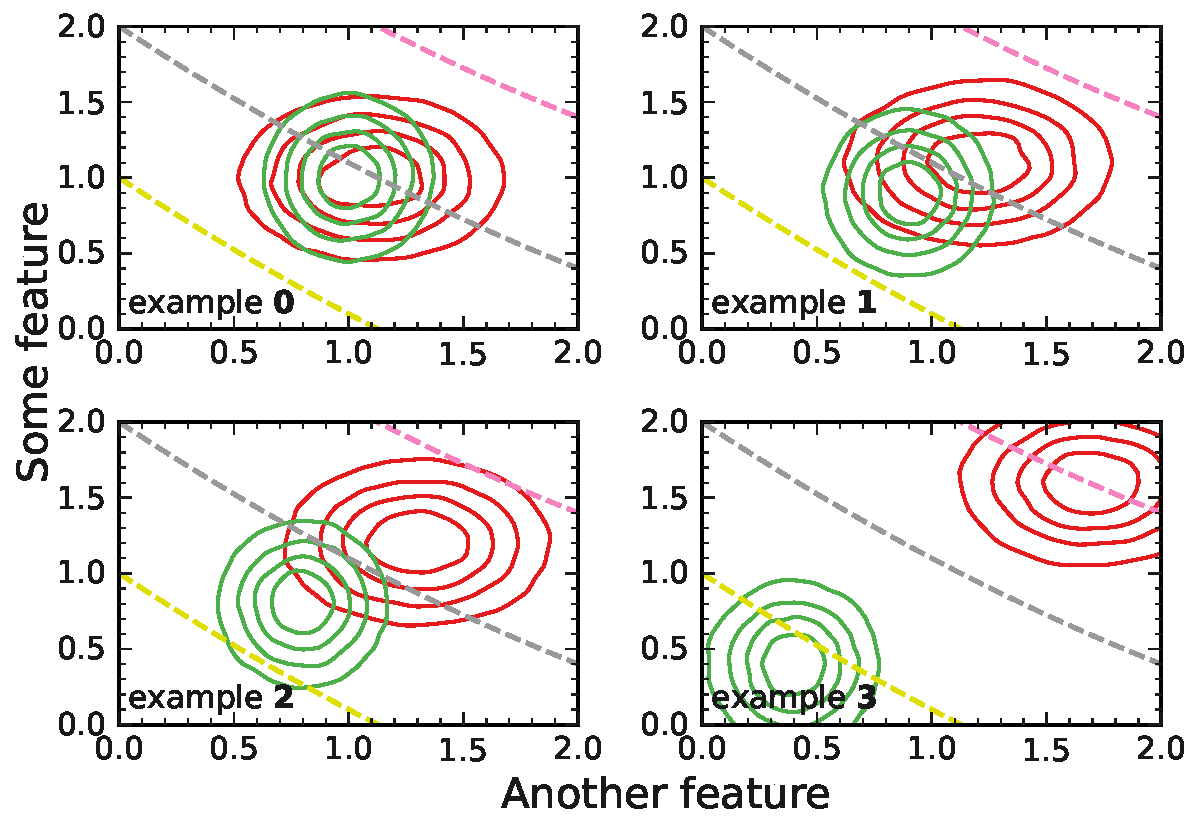
\includegraphics[width=0.45\textwidth]{figures/analysis_techniques/separation_boundary.pdf}
        }
    \subcaptionbox{\label{fig:roc_curves}}{
    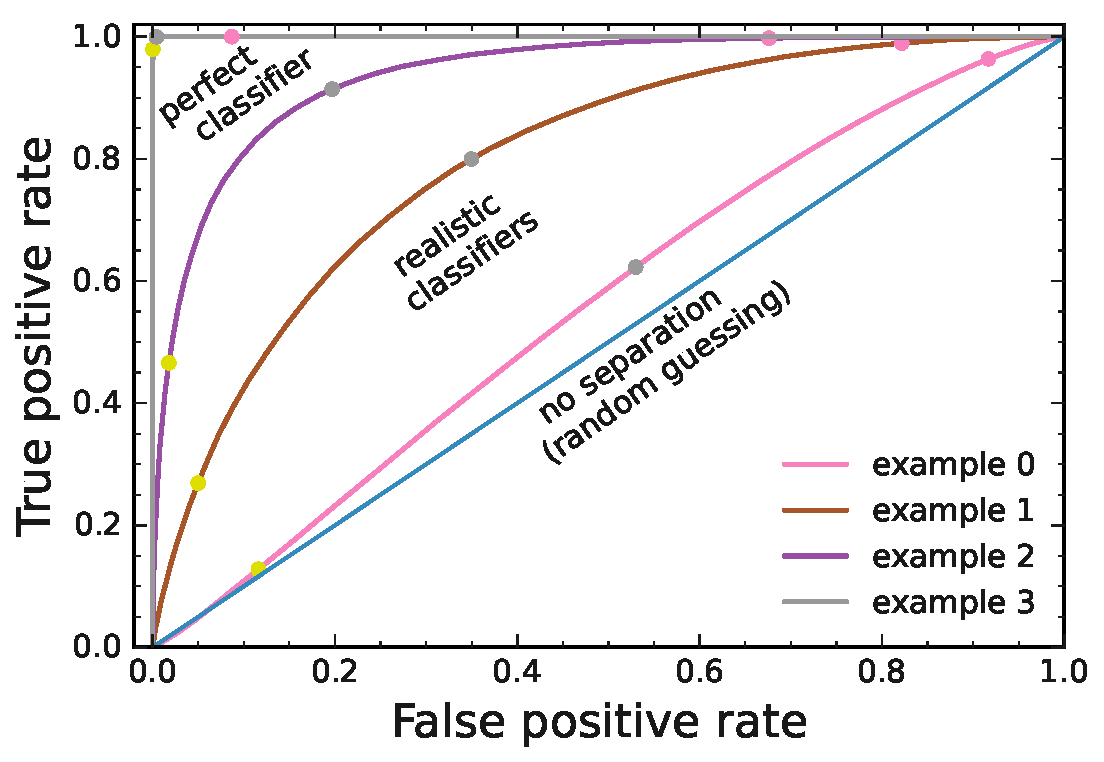
\includegraphics[width=0.45\textwidth]{figures/analysis_techniques/roc_curve.pdf}
    }
    \caption{\label{fig:rocs_examples}
    Two-dimensional distributions (red/green) in two-feature space are shown in \Cref{fig:distributions_separation} for four different examples (0-3).
    Each distribution is represented by a contour-plot of 20\% isoproportion lines.
    Dashed lines show the examples for different selection thresholds for an example \MVA model.
    \Cref{fig:roc_curves} shows corresponding \ROC curves, calculated for examples 0-3.
    The working points that represent the dashed lines of \Cref{fig:distributions_separation} are shown in the same color, for each of the four curves.
    A perfect classifier would be able to perfectly separate green and red distributions, similar to example~3.
    On the other hand, a poor classifier would only be able to perform marginally better than random-guessing, similar to example~0.    
    }
\end{figure}


To assess the performance of a binary classifier, a receiver operating characteristic (\ROC) is often used.
A \ROC curve represents the true-positive rate as a function of the false-positive rate and is calculated by iterating over different \MVA classifier selections.
A visual representation of the meaning of \ROC curves is shown in \Cref{fig:rocs_examples}.
Given an optimal training, one expects the \ROC curve calculated on training and testing data to be highly similar.
This can be qualitatively by visually inspecting the corresponding curves, or, quantitatively, by defining an area-under-curve (\AUC) score which is computed by integrating the \ROC curve.
An $\mathrm{\AUC}=1$ would represent false-positive rate of 0, and a true-positive rate of 1 (see \Cref{fig:roc_curves})
The least-optimal classifier would provide a random guess and have a false-positive and true-positive rate of 0.5, and $\mathrm{\AUC}=0.5$.

In high-energy physics, we often use alternative forms of false-positive and true-positive rates.
Namely, we tend to express our results in terms of 
\begin{itemize}
    \item \textit{efficiency}: equivalent to the true-positive rate;
    \item \textit{background rejection}: equivalent to $1 - \mathrm{false-positive~rate}$;
    \item \textit{purity}: amount of signal, with respect to the total sample size (signal+background); equivalent to positive-predictive value.
\end{itemize}

\subsection{(Boosted) decision trees}\label{sec:BDTs_theory}

When combining many different features together, selecting an appropriately parametrised model (\Cref{eq:loss_function}) can be complicated and sub-optimal.
Therefore, non-parametric models are often desired, and a simple way to implement these are \textit{decision trees}.

A decision tree is a classification technique where the $N$-dimensional feature space is divided based on a series of binary selections.
A simple model (often a constant) is used to make a split in each of the feature space regions, and the splitting process is then repeated on the two resulting regions.
The exact value to split by is optimised in each region independently.
For classification problems cross-entropy is common to be used as a loss-function:
\begin{equation}
    \mathcal{L}(y,\hat{y})=-\sum_{j=1}^J y_j\log \hat{y}_j + (1-y_j)\log(1-\hat{y}_j),
\end{equation}
where $y$ is a target and $y_j$ is a predicted label.
Each final region which has not been sub-splitted is called a \textit{leaf}.
A set of selections leading to a leaf is known as a \textit{branch}. 
Therefore at the end of every branch there is a node with two leaves.
The maximum number of selections in a branch is called the \textit{depth} of the classifier.


The tree could be grown indefinitely and it is obvious that this will quickly lead to overtraining, highlighting the aforementioned bias-variance trade-off.
In practice, a technique called \textit{pruning} is employed, which removes nodes from the tree based on their overall impact on the performance of the decision tree.
This produces a smaller tree and the `strength' of pruning is tunable with appropriate parameters.

Decision trees are easily interpretable as they mimic human logic in terms of a number of sequential binary decisions.
However, they also tend to be highly-dependant on the statistical fluctuations of the training dataset.
With pruning, their performance on independant samples usually turns out to be weaker than many other MVAs, and the misclassification rate only slightly better than random guesses.
A single decision tree is, therefore, considered a \textit{weak classifier}.

This and other problems surrounding decision trees are addressed by employing \textit{boosting} and forming boosted decision trees (\BDT{s}).
Boosting enhances the performance of an ensemble of weak classifiers by combining their output. 
The performance of such a boosted ensemble can be much better even when all the input classifiers are weak.

During the first training iteration of a \BDT, a regular decision tree would be trained, as explained before, with a shallow limit on the depth.
However, after that there would follow a second training iteration, where the events that were misclassified in the last training iteration are given a larger weight.
The procedure is repeated $M$ times to train a set of classifiers $g_{m}(x)$, where $m=1,2,..,M$.
The final output is a weighted `majority-vote' of all these classifiers:
\begin{equation}\label{eq:boosted_classifier}
    G(x) = \sum_{m=1}^M\alpha_mg_m(x),
\end{equation}
with $\alpha_m$ being the weight of the $m$-th weak classifier.
Conventionally, the output of the classifier is transformed, such that $G(x)\ra G'(x)\in[0,1]$.

The exact procedure to assign weights to misclassified events between training iterations and the computation of $\alpha_m$ depends on the boosting technique used.
Consider an initial guess $G_1$, which corresponds to $M=1$ case in \Cref{eq:boosted_classifier}.
One can then, given some learning rate (\textit{shrinkage}) $0<\nu\leq1$, update the prediction with every training iteration:
\begin{equation}
    G_m(x) = G_{m-1}(x) + \nu\alpha_mg_m(x),
\end{equation}
by minimising the loss function for parameter $\alpha_m$: 
\begin{equation}\label{eq:minimize_loss}
    \alpha_m = \arg\min_{\alpha_m}\left(\sum_{i=1}^N\mathcal{L}(y_i, G_{m-1}(x_i) + \alpha_mg_m(x_i))\right).
\end{equation}
One way to solve \Cref{eq:minimize_loss} in a numerically-optimal way is to compute the gradient of the loss function.
Consequentially, a classifier built this way is called \textit{gradient-boosted} decision tree \cite{FRIEDMAN1013203451}.

To further increase robustness of gradient-\BDT{s}, one may only sample (without replacement) a part of the dataset in each training iteration.
In this case, any statistical fluctuations would average out over the sum of all trees. 
This technique is called stochastic gradient-\BDT{s} \cite{FRIEDMAN2002367}.
The fraction of data used at every training iteration is called the \textit{sampling rate}.

In the analyses present in this thesis, \texttt{FastBDT} \cite{Keck:2017gsv} is used as the \MVA for training stochastic gradient-\BDT{s}.
For the training of the classifier, \texttt{FastBDT} employs 4 parameters that were described in this chapter: number of trees ($M$), maximum depth of each tree, shrinkage and sampling rate. 

\section{Unfolding}\label{sec:unfolding}

In physics, we are only able to probe Nature through the experimental setup that we build.
Any hypothethical detector is therefore subjected to random effects related to the finite resolution and acceptance of the detector.
Consequentially, the measured results (distributions) will be convoluted with these effects (\textit{smeared}).
If two different experiments are comparing their measurements, it only makes sense if external factors are of minimal importance.
The process of deconvoluting the true distribution from the measured distribution is called \textit{unfolding}.
In this way, it can be considered the `opposite' of measurement.

This section provides a brief overview of the main concepts that feature in the results presenting this thesis.
A thorough summary of the theory behind unfolding methods can be found in \cite{Behnke:2013pga,Blobel_Lohrmann_1998} and a comparison of different methodologies common in particle physics in \cite{Schmitt:2016orm,Cowan:2002in,Brenner:2019lmf}.

\subsection{Mathematical basis}

Consider a true distribution $f(x)$ of observable $x$ being measured in some space $a<x<b$.
The corresponding measured distribution $g(y)$ as a function of the measured value $y$ is related to $f(x)$ as:
\begin{equation}\label{eq:fredholm_integral}
    g(y) =  \int_a^b A(y,x) f(x) dx,
\end{equation}
which is the Fredholm intergral equation of the first kind \cite{Blobel_Lohrmann_1998}.
The function $A(y, x)$ is the Kernel (or response) function, and it holds the information about physical nature of the measurement.
In the process of unfolding, one seeks to find $f(x)$ given $g(y)$.
Such a problem does not have a general solution and in the cases when there is a solution it can be highly dependant on small changes in $g(y)$ \cite{Delves_Walsh_1974}.
\Cref{fig:smearing_illustration} visually illustrates the smearing of a true distribution for an arbitrary observable given two smearing effects.
These effects, which would contribute to the form of the $A(y,x)$, are unknown in reality.
The main method in high-energy physics is to extract an implicit form of this function from simulated-samples.

\begin{figure}[htbp!]
    \centering
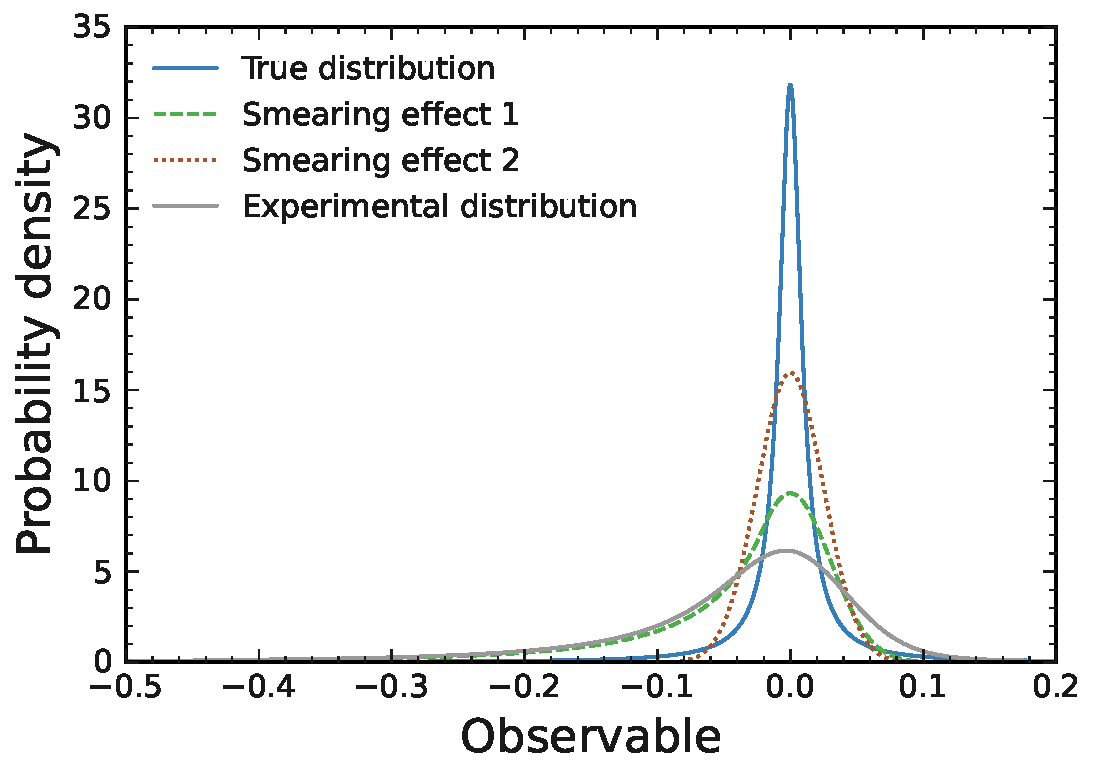
\includegraphics[width=0.45\textwidth]{figures/analysis_techniques/experimental_smearing.pdf}
\caption{\label{fig:smearing_illustration} A visual illustration of smearing of an arbitrary observable.
Considering some `true' distribution (blue, full line), depicted by a sharp Lorentzian, the experimentally observed result (gray, full line) will be affected by, usually, unknown detector-response and resolution effects.
In this case, the unknown-experimental effects are illustrated by a Gaussian (dotted) and Crystal Ball (dashed) functions.}
\end{figure}

In science, experimental data are often presented in the form of a histogram. 
In that case the results are integrated over several shorter intervals (\textit{bins}) and only the integral values are shown at the center of each bin.
As a result, a simpler matrix form of \Cref{eq:fredholm_integral} can be used which allows a numerical solution:
\begin{equation}\label{eq:unfolding_linear_equation}
\hat{A}\vec{x}=\vec{y},
\end{equation}
where:
\begin{itemize}
    \item $\vec{x}$ is an $m$-dimensional vector of binned unknown true distribution;
    \item $\vec{y}$ is an $n$-dimensional vector of binned measured distribution;
    \item $\hat{A}$ is an $n\times m$-dimensional response matrix.

\end{itemize}
In general, \Cref{eq:fredholm_integral,eq:unfolding_linear_equation} may contain additional terms dependant on $y$ corresponding to background contributions and statistical fluctuations.

The elements $A_{ij}$ of $\hat{A}$ correspond to a probability to measure an event in bin-$j$ that was produced in bin-$i$.
In particle physics, the response matrix is generally built using Monte Carlo simulated samples that generate a particle collisions, simulate signal processing and detector effects.
By taking the ratio of simulated events generated in a bin $i$, $N_i^{\mathrm{gen}}$, with the number of simulated events that were generated in bin $j$ but were measured in bin $i$, $N_{ij}^{\mathrm{meas}}$:
\begin{equation}\label{eq:response_matrix_element}
    A_{ij} = \frac{N_{ij}^{\mathrm{meas}}}{N_i^{\mathrm{gen}}}.
\end{equation}
There are a number of methods solve \Cref{eq:unfolding_linear_equation}, discussed in the following sections.

\subsection{Bin-by-bin unfolding}

The simplest approach is to scale the measured distribution in each bin $i$ by a factor determined from simulation:
\begin{equation}\label{eq:bin_by_bin_unfolding}
 x_i = y_i \times \frac{N_i^{\mathrm{gen}}}{N_i^{\mathrm{meas}}},
\end{equation}
where $N_i^{\mathrm{meas}}$ is $\sum_j N_{ij}^{\mathrm{meas}}$.
It follows that uncertainties propagate trivially:
\begin{equation}\label{eq:bin_by_bin_unfolding_error}
    \Delta x_i = \Delta y_i \times \frac{N_i^{\mathrm{gen}}}{N_i^{\mathrm{meas}}},
\end{equation}
where $\Delta x_i$ and $\Delta y_i$ are uncertainties associated with these quantities.

This method is only possible if the number of bins in the true distribution is equal to the number of bins in the measured distribution.
Furthermore, it does not take any cross-bin effects into account, i.e. effectively treats each bin as uncorrelated.
Therefore, it is usually used when the necessary corrections are small or when the statistical uncertainty dominates the experimental result.
The method is referred to as \textit{bin-by-bin} unfolding, or bin-by-bin correction method.
It has been the main method applied in the works of this thesis.

\subsection{Matrix inversion method}
The matrix inversion method is the simplest method which does not include assumptions about the measured data (e.g. uncorrelated bins).
In this case the \Cref{eq:unfolding_linear_equation} is solved by inverting the response matrix:
\begin{equation}
    \vec{x} = \hat{A}^{-1}\vec{y}.
\end{equation}
The number of bins of the true and the measured distribution must be the same, as only square matrices may be inverted.
While the result is statistically fully correct, it tends to introduce large negative correlations between neighbouring bins in the unfolded distribution $\vec{x}$ \cite{Schmitt:2016orm}.
The simple reasoning for this is the fact that poissonian fluctuations in neighbouring bins will get amplified/suppressed by the matrix multiplication, creating an``oscillatory'' pattern.
This effect is undesirable and goes against the common sense as smooth distributions are expected in nature.
The correction of such correlations is called \textit{regularisation}.
The effect of regularisation is shown in XX

\subsection{Other unfolding methods and regularisation}
As discussed in the last subsection, unfolding introduces large correlations, leading to `non-physical' shapes of unfolded distributions.
Regularisation is a very delicate task because, roughly put, the scientist has a prejudice towards smooth measured distribution and therefore artificially adds a bias to smoothen it.
Unsurprisingly, there are many different methods to perform this.
Although an in-depth discussion is irrelevant for the purpose of the works presented in this thesis, some of the most common ones in particle physics are listed here:
\begin{itemize}
    \item \texttt{TUnfold} method \cite{Schmitt:2012kp}: performs a least-squares minimisation of $\vec{y}-\hat{A}{\vec{x}}$ and includes a damping term for oscillations in $x$;
    \item D'Agostini method \cite{d2010improved,DAgostini:1994fjx}: inversion of response matrix using Bayes' theorem and iterative improvement of the unfolding result, stopping iterations early to not require regularisation;
    \item Iterative dynamically-stabilised method \cite{Malaescu:2009dm}: combines elements of d'Agostini's and bin-by-bin correction methods, preserving the normalisation of data in each bin;
    \item Singular value decomposition method \cite{Hocker:1995kb}: solves \Cref{eq:unfolding_linear_equation} by decomposing the response matrix into its singular values, adds a weighted prior condition to the solution.
\end{itemize}
In particle physics, unfolding is often implemented using the \texttt{RooUnfold} package \cite{Brenner:2019lmf}, which can perform all the methods described in \Cref{sec:unfolding}.
In the analyses present in this thesis, regularisation was no applied.

\section{Blinded analysis}\label{sec:blinding}

In order to avoid an experimenter's bias analyses are often performed in a \textit{blinded} way \cite{Roodman:2003rw}.
The bias can occur when using the analysed data directly to perform optimisations or compare several different techniques.
An experimenter, uninentionally, may enhance statistical or unknown-systematic effects which bias the sample to give a desired or expected result.
Generally, one restricts access to the analysed sample until after the measurement setup is prepared.
In particle physics, this is done by performing the analysis on simulated data, and then using independent data-samples to perform checks that the analysis is behaving as appropriate.
Normally, a certain range of an interesting observable is hidden, for example, in the case of \BtoXsgamma analysis presented here, it can be the photon energy, \Egamma.
This method is well-suited when performing measurements where the signal region is known in advance, as is the case in the example I mentioned.
The removal of a constraint and the application the analysis technique on real data is called \textit{unblinding}.
It is usually performed as the last step, once other steps in the analysis have been scrutinised and validated.
This is also the procedure that was applied in the inclusive \BtoXsgamma studies described in this thesis.